\documentclass{article}

\usepackage{graphicx}
\usepackage{subcaption}
\usepackage[hypcap]{caption}
\usepackage{listings}

\title{Experimental Design and Data Analysis: Assignment 1}
\author{Andrew Bedard(10860606) \& Simone van Gompel(2567525) \\ Group 19}

\begin{document}

  \maketitle

  \section{Exercise 1}
    For the data in X1 and X4 we cannot say with certainty that it is normally distributed, and looking at a QQ-plot for a random normal dataset of the same size does not help much in determining whether they are normally distributed. This can be seen in Fig:\ref{fig:X1} and Fig:\ref{fig:X4}.\\
    It is clear that the data in X2 and X5 are not normally distributed, this can be seen by comparing the QQ-plots of normally distributed data of the same size, which gives a much more distinct straight line than X2, X5.
    See this in Fig:\ref{fig:X2} and Fig:\ref{fig:X5}.\\
    The data X3 is likely normally distributed, this can be seen by the shape of the histogram which roughly looks like a normal distribution. Further the QQ-plot produces a clear straight line with few exceptions, similar to the QQ-plot of the normally distributed random data of the same size.
    See this in Fig:\ref{fig:X3}.\\
    See the used code in:\ref{sub:R1}

    \begin{figure}
    \begin{subfigure}{.5\textwidth}
      \centering
      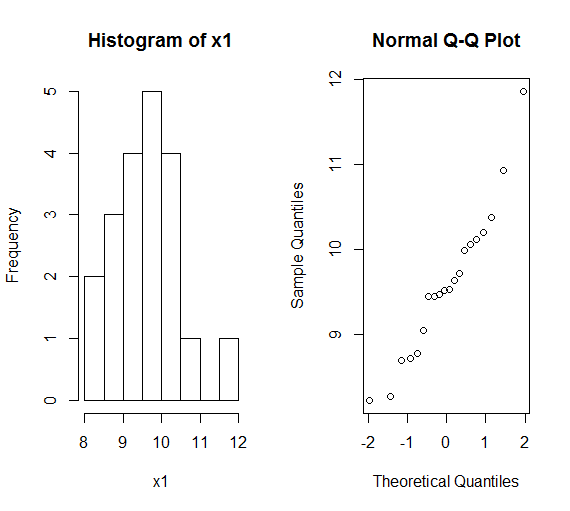
\includegraphics[width=.8\linewidth]{results/X1}
      \caption{X1 Data}
    \end{subfigure}
    \begin{subfigure}{.5\textwidth}
      \centering
      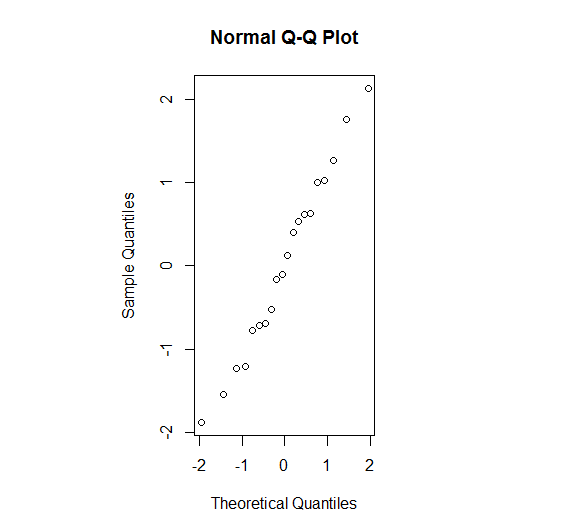
\includegraphics[width=.8\linewidth]{results/X1_2}
      \caption{Rnorm data of same size}
    \end{subfigure}
    \caption{X1}
    \label{fig:X1}
    \end{figure}

    \begin{figure}
    \begin{subfigure}{.5\textwidth}
      \centering
      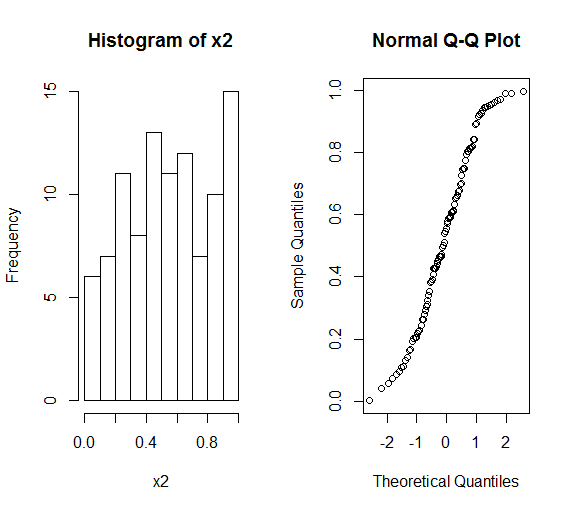
\includegraphics[width=.8\linewidth]{results/X2}
      \caption{X2 Data}
    \end{subfigure}
    \begin{subfigure}{.5\textwidth}
      \centering
      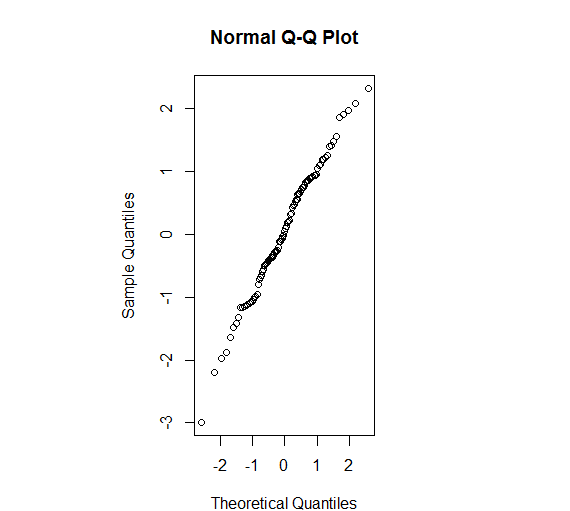
\includegraphics[width=.8\linewidth]{results/X2_2}
      \caption{Rnorm data of same size}
    \end{subfigure}
    \caption{X2}
    \label{fig:X2}
    \end{figure}

    \begin{figure}
    \begin{subfigure}{.5\textwidth}
      \centering
      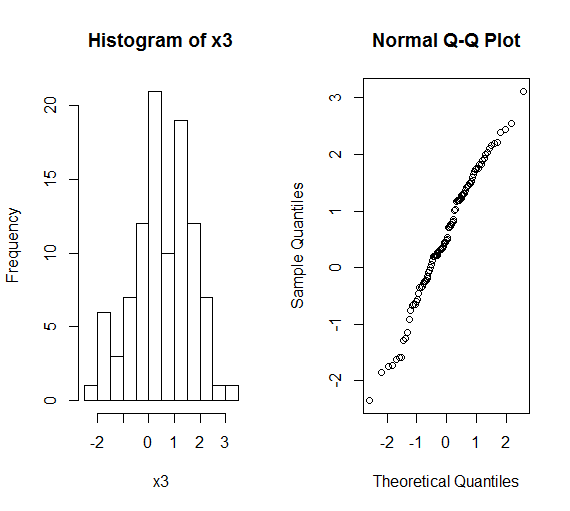
\includegraphics[width=.8\linewidth]{results/X3}
      \caption{X3 Data}
    \end{subfigure}
    \begin{subfigure}{.5\textwidth}
      \centering
      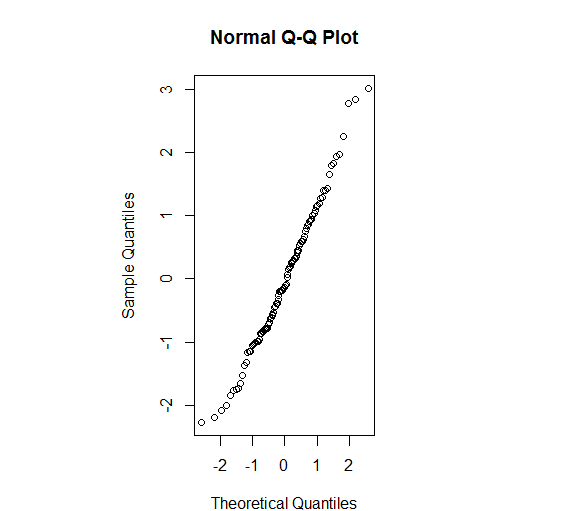
\includegraphics[width=.8\linewidth]{results/X3_2}
      \caption{Rnorm data of same size}
    \end{subfigure}
    \caption{X3}
    \label{fig:X3}
    \end{figure}

    \begin{figure}
    \begin{subfigure}{.5\textwidth}
      \centering
      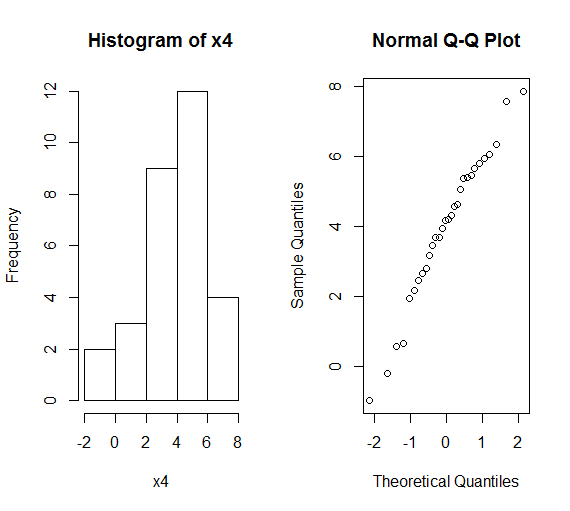
\includegraphics[width=.8\linewidth]{results/X4}
      \caption{X4 Data}
    \end{subfigure}
    \begin{subfigure}{.5\textwidth}
      \centering
      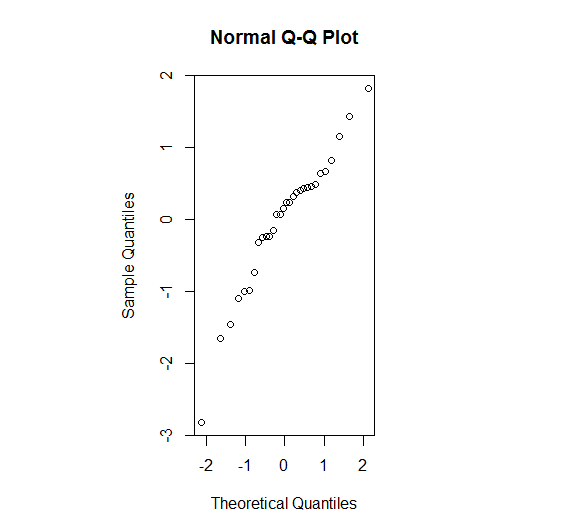
\includegraphics[width=.8\linewidth]{results/X4_2}
      \caption{Rnorm data of same size}
    \end{subfigure}
    \caption{X4}
    \label{fig:X4}
    \end{figure}

    \begin{figure}
    \begin{subfigure}{.5\textwidth}
      \centering
      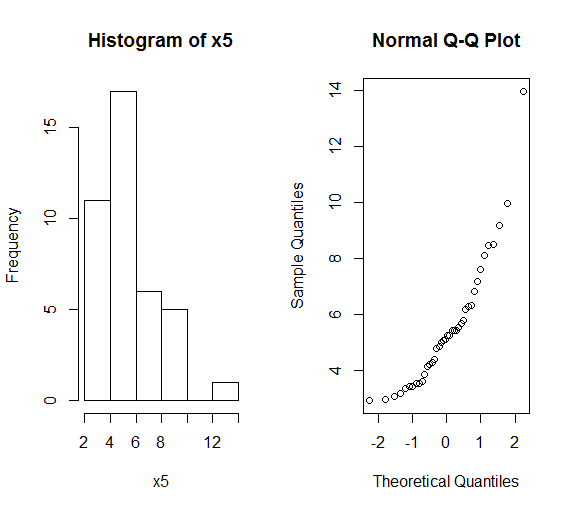
\includegraphics[width=.8\linewidth]{results/X5}
      \caption{X5 Data}
    \end{subfigure}
    \begin{subfigure}{.5\textwidth}
      \centering
      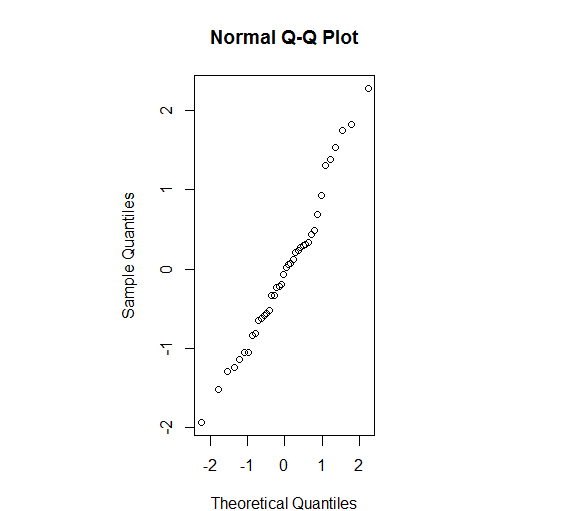
\includegraphics[width=.8\linewidth]{results/X5_2}
      \caption{Rnorm data of same size}
    \end{subfigure}
    \caption{X5}
    \label{fig:X5}
    \end{figure}

  \section{Exercise 2}

    \subsection{2.1}
      After running the simulation the following results were obtained:
      \begin{itemize}
        \item Number of p-values smaller than 5\%: 44
        \item Number of p-values smaller than 10\%: 93
        \item The histogram and QQ-Plot Fig:\ref{fig:2_1}
      \end{itemize}

      \begin{figure}[!htb]
      \begin{subfigure}{.5\textwidth}
        \centering
        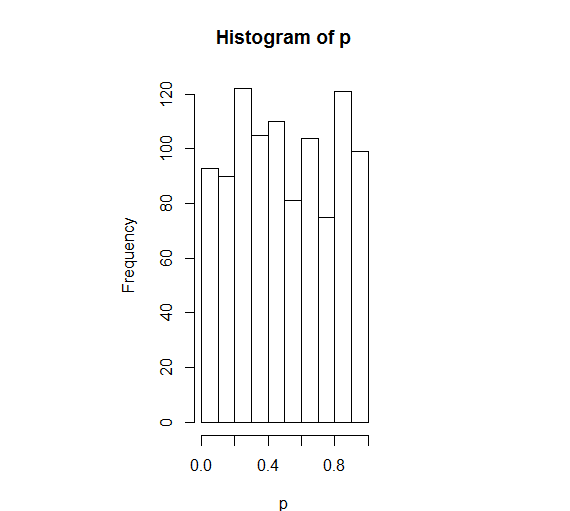
\includegraphics[width=.8\linewidth]{results/2_1}
        \caption{Histogram p-values}
        \end{subfigure}
        \begin{subfigure}{.5\textwidth}
        \centering
        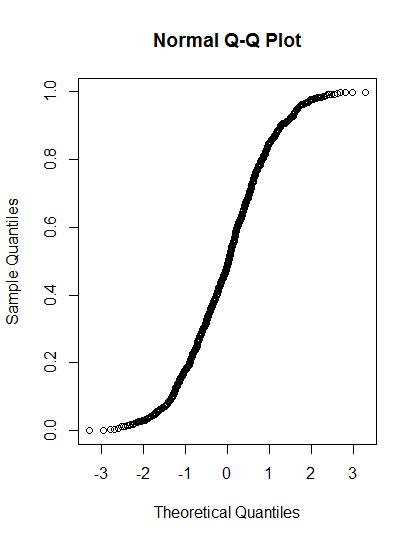
\includegraphics[width=.8\linewidth]{results/2_1_2}
        \caption{QQ-plot p-values}
        \end{subfigure}
        \caption{}
        \label{fig:2_1}
      \end{figure}
      
      It is clear from both the histogram and the QQ-plot of the p-values, that this is roughly uniformly distributed. This is also obvious when comparing against the QQ-plot of a random uniform dataset of the same size, which can be seen in figure \ref{fig:2_uniform}. The QQ-plot of our p-values and the random uniform values are indistinguishable to the naked eye.
      
      \begin{figure}[!htb]
      \centering
      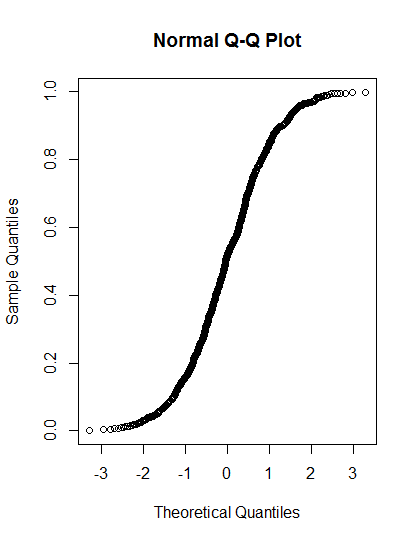
\includegraphics[scale=0.5]{results/2_discussion}
      \caption{QQ-Plot of Random Uniform dataset of 1000 values}
      \label{fig:2_uniform}
      \end{figure}

    \subsection{2.2}
      After running the simulation the following results were obtained:
      \begin{itemize}
        \item Number of p-values smaller than 5\%: 52
        \item Number of p-values smaller than 10\%: 106
        \item The histogram and QQ-Plot Fig:\ref{fig:2_2}
      \end{itemize}
      
      \begin{figure}[!htb]
      \begin{subfigure}{.5\textwidth}
        \centering
        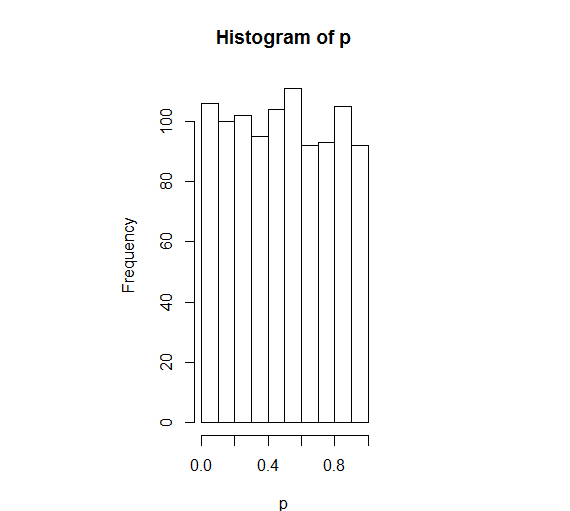
\includegraphics[width=.8\linewidth]{results/2_2}
        \caption{Histogram p-values}
        \end{subfigure}
        \begin{subfigure}{.5\textwidth}
        \centering
        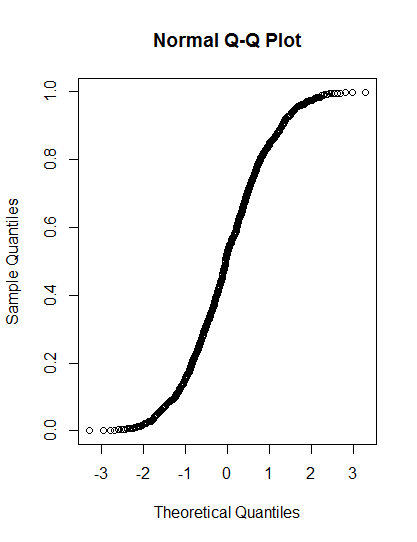
\includegraphics[width=.8\linewidth]{results/2_2_2}
        \caption{QQ-plot p-values}
        \end{subfigure}
        \caption{}
        \label{fig:2_2}
      \end{figure}
      
      It is clear that the results are very similar to those of the previous question. Once again both the histogram and the QQ-Plot suggest that the p-values are uniformly distributed.

\newpage
    \subsection{2.3}
      After running the simulation the following results were obtained:
      \begin{itemize}
        \item Number of p-values smaller than 5\%: 966
        \item Number of p-values smaller than 10\%: 984
        \item The histogram and QQ-Plot Fig:\ref{fig:2_3}
      \end{itemize}
      
      \begin{figure}[!htb]
      \begin{subfigure}{.5\textwidth}
        \centering
        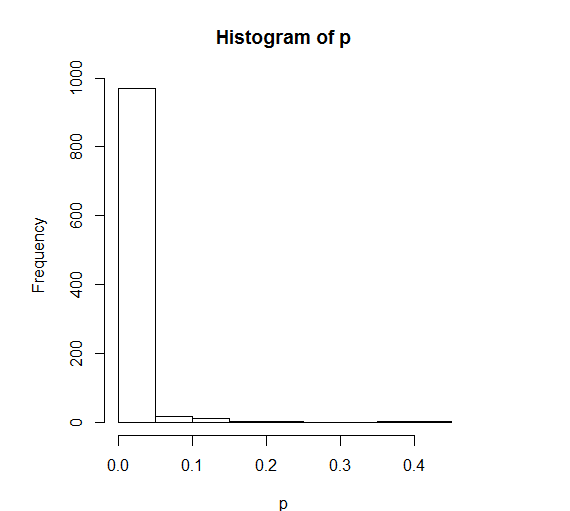
\includegraphics[width=.8\linewidth]{results/2_3}
        \caption{Histogram p-values}
        \end{subfigure}
        \begin{subfigure}{.5\textwidth}
        \centering
        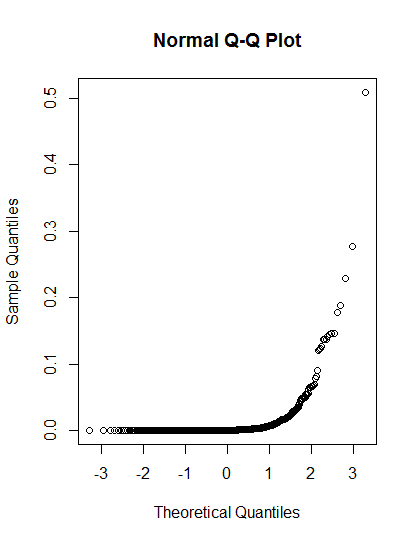
\includegraphics[width=.8\linewidth]{results/2_3_2}
        \caption{QQ-plot p-values}
        \end{subfigure}
        \caption{}
        \label{fig:2_3}
      \end{figure}
      
      From the histogram and QQ-plot of this data it was far less clear what type of distribution is being represented. It is clear at least that it is heavily right skewed.
      
\newpage
    \subsection{2.4}
      The results are unsurprising when you consider what we are actually testing. Clearly the distribution of the p-values will be roughly uniform if we are comparing two data sets with identical population sizes (m and n) and identical means (mu and nu). In the terms of the t-test, we have a relatively small number of p-values which suggest we reject the null hypothesis, therefore the populations are roughly equal. Further, the standard deviation should have no effect on the results when comparing two nearly identical data sets, as was seen with the lack of difference between the histograms and QQ-Plots generated in \textbf{2.1} and \textbf{2.2}
      
      Different results obtained in part \textbf{2.3} were different because the sample means were changed. The t-test was then able to distinguish between the data sets a majority of the time, in other words, the fact that we had so many p-values less than 0.05 suggests that we should reject the null hypothesis, which in this case was that the two populations were identical.
      
\newpage
  \section{Exercise 3}
  The following figure was created from the code outline in the appendix. The red points are the values of the power of the t-test based on parameters outline in section \textbf{3.1}, blue points are values based on section \textbf{3.2}, and the green points from section \textbf{3.3}
      See Fig:\ref{fig:3_1}.
      \begin{figure}[!htb]
        \centering
        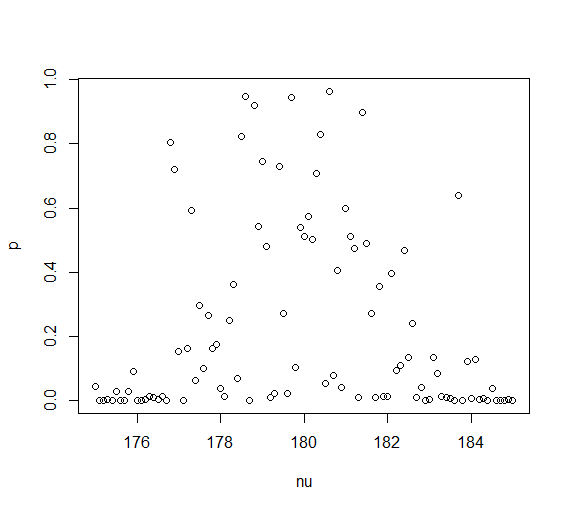
\includegraphics[width=.8\linewidth]{results/3_1}
        \caption{Powers as a function of nu}
        \label{fig:3_1}
      \end{figure}


    \subsection{3.4}
      The figure obtained in this exercise gives an idea of how the t-test is able to differentiate two data sets. For example, the red points were obtained from a smaller population than the blue points, so naturally if the data is not perfectly uniform this will have a larger affect on the smaller population in the form of false negatives, that is, the t-test being less discerning with smaller populations and subtle changes in sample means. The data in blue shows that the Power of the t-test is very quick to detect differences in the samples with a larger population size.
      
      The green points, which were obtained by dramatically increasing the standard deviation are very interesting, but once again their meaning is intuitive. When the standard deviation is so large compared to the values we are examining, then the variance of the values will also be large. This means simply that even though two sample sets may have the same mean, the variance almost certainly insures that they will appear to be from completely different sets, which the t-test recognises in the form of false positives, and powers that consistently suggest that we reject the null hypothesis
\newpage
  \section{R-Code}
    \subsection{Exercise 1}\label{sub:R1}
      \begin{lstlisting}[language=R]
        load(file="assign1.RData")

        par(mfrow=c(1,2))
        hist(x1)
        qqnorm(x1)

        hist(x2)
        qqnorm(x2)

        hist(x3)
        qqnorm(x3)

        hist(x4)
        qqnorm(x4)

        hist(x5)
        qqnorm(x5)

        par(mfrow=c(1,1))
        par(pin=c(2.5,5))
        qqnorm(rnorm(20))
        qqnorm(rnorm(100))
        qqnorm(rnorm(100))
        qqnorm(rnorm(30))
        qqnorm(rnorm(40))
      \end{lstlisting}

    \subsection{Exercise 2}\label{sub:R2}
      \begin{lstlisting}[language=R]
        #2.1
        m=30
        n=30
        mu=180
        nu=180
        sd=10
        B=1000
        p=numeric(B)

        for (b in 1:B) {
          x=rnorm(m,mu,sd)
          y=rnorm(n,nu,sd)
          p[b]=t.test(x,y,var.equal=TRUE)[[3]]
        }

        sum(p<0.05)
        sum(p<0.1)
        par(pin=c(5,5))
        hist(p)
        qqnorm(p)

        #2.2
        sd=1
        p=numeric(B)

        for (b in 1:B) {
          x=rnorm(m,mu,sd)
          y=rnorm(n,nu,sd)
          p[b]=t.test(x,y,var.equal=TRUE)[[3]]
        }

        sum(p<0.05)
        sum(p<0.1)
        hist(p)
        qqnorm(p)

        #2.3
        nu=175
        sd=5
        p=numeric(B)

        for (b in 1:B) {
          x=rnorm(m,mu,sd)
          y=rnorm(n,nu,sd)
          p[b]=t.test(x,y,var.equal=TRUE)[[3]]
        }

        sum(p<0.05)
        sum(p<0.1)
        hist(p)
        qqnorm(p)
      \end{lstlisting}

    \subsection{Exercise 3}\label{sub:R3}
      \begin{lstlisting}[language=R]
        #3.1
        mu=180
nu=seq(175,185,by=0.1)
m=30
n=30
sd=5
B=1000
p=numeric(B)
dummy=0
powers1=numeric(length(nu))
for (nu_tmp in nu){
  dummy=dummy+1
for (b in 1:B) {
  x=rnorm(m,mu,sd)
y = rnorm(n,nu_tmp,sd)
p[b]=t.test(x,y,var.equal=TRUE)[[3]]}
powers1[dummy]=mean(p<0.05)}


        #3.2
mu=180
nu=seq(175,185,by=0.1)
m=100
n=100
sd=5
B=1000
p=numeric(B)
dummy=0
powers2=numeric(length(nu))
for (nu_tmp in nu){
  dummy=dummy+1
for (b in 1:B) {
  x=rnorm(m,mu,sd)
y = rnorm(n,nu_tmp,sd)
p[b]=t.test(x,y,var.equal=TRUE)[[3]]}
powers2[dummy]=mean(p<0.05)}


        #3.3
mu=180
nu=seq(175,185,by=0.1)
m=30
n=30
sd=100
B=1000
p=numeric(B)
dummy=0
powers3=numeric(length(nu))
for (nu_tmp in nu){
  dummy=dummy+1
for (b in 1:B) {
  x=rnorm(m,mu,sd)
y = rnorm(n,nu_tmp,sd)
p[b]=t.test(x,y,var.equal=TRUE)[[3]]}
powers3[dummy]=mean(p<0.05)}

plot(nu,powers1,col="red")
points(nu,powers2,col="blue")
points(nu,powers3,col="green")
      \end{lstlisting}

\end{document}